% Created by tikzDevice version 0.7.0 on 2015-01-23 13:36:45
% !TEX encoding = UTF-8 Unicode
\documentclass[10pt,twoside]{book}\usepackage[T1]{fontenc}
\usepackage{tikz}

\usepackage[active,tightpage,xetex]{preview}

\usepackage{fontspec,xunicode}

\PreviewEnvironment{pgfpicture}

\setlength\PreviewBorder{0pt}

\usetikzlibrary{calc}

\usetikzlibrary{positioning}



\usepackage{fontspec,xunicode}

\setmainfont{Open Sans Condensed Light}
\begin{document}
\begin{tikzpicture}
\node[anchor=south west,inner sep=0] (image) at (0,0) {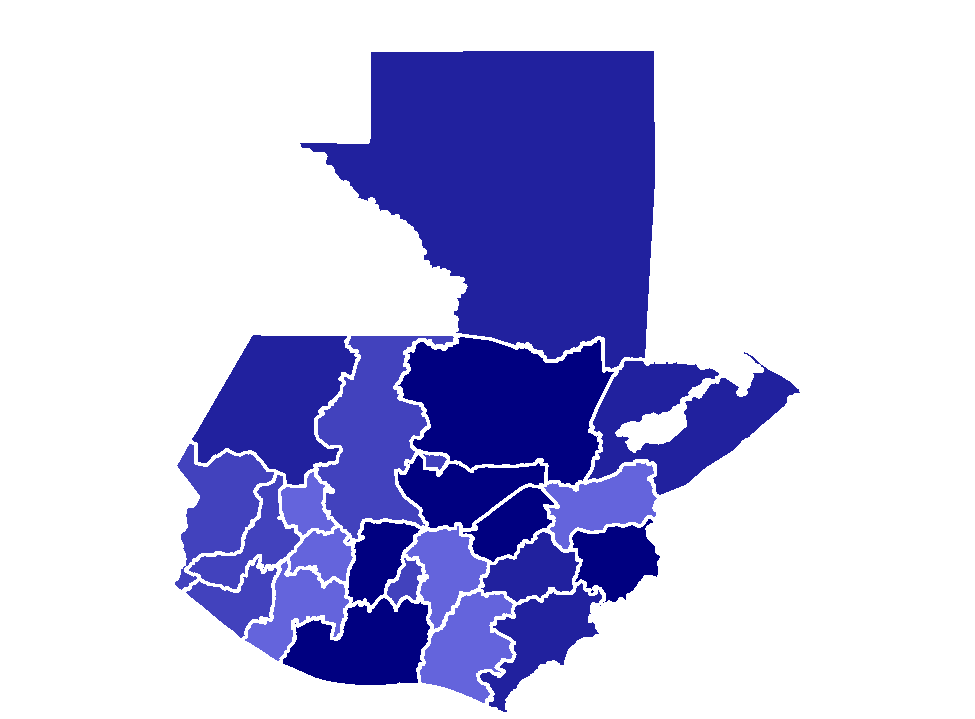
\includegraphics{mapa}};
\begin{scope}[x={(image.south east)},y={(image.north west)}]
\draw[help lines,xstep=.1,ystep=.1] (0,0) grid (1,1);
\foreach \x in {0,1,...,9} { \node [anchor=north] at (\x/10,0) {0.\x}; }
\foreach \y in {0,1,...,9} { \node [anchor=east] at (0,\y/10) {0.\y}; }
% ###############ALTA VERAPAZ############################## %
\draw [thick] (0.5,0.4) -- (0.5,0.9);
\filldraw (0.5,0.4) circle (1pt);
\draw [thick] (0.4989,0.9) -- (0.73,0.9);
\node[text width=3cm] at (0.83,0.9) {Alta Verapaz \\ 5\%};

% ###############BAJA VERAPAZ############################## %
\draw [thick] (0.5,0.4) -- (0.5,0.9);
\filldraw (0.5,0.4) circle (1pt);
\draw [thick] (0.4989,0.9) -- (0.73,0.9);
\node[text width=3cm] at (0.83,0.9) {Alta Verapaz \\ 5\%};

% ###############PETEN############################## %
\draw [thick] (0.58,0.55) -- (0.58,0.67);
\filldraw (0.58,0.55) circle (1pt);
\draw [thick] (0.5789,0.67) -- (0.73,0.67);
\node[text width=3cm] at (0.83,0.67) {Petén \\ 5\%};

%#############IZABAL################################# %
\draw [thick] (0.64,0.45) -- (0.64,0.55);
\filldraw (0.64,0.45) circle (1pt);
\draw [thick] (0.6389,0.55) -- (0.73,0.55);
\node[text width=3cm] at (0.83,0.55) {Izabal \\ 5\%};

%#############EL PROGRESO################################# %
\draw [thick] (0.55,0.28) -- (0.55,0.75);
\filldraw (0.55,0.28) circle (1pt);
\draw [thick] (0.6389,0.55) -- (0.73,0.55);
\node[text width=3cm] at (0.83,0.55) {El Progreso \\ 5\%};
\end{scope}
\end{tikzpicture}
\end{document}
